\documentclass{beamer}
% Use the following three lines instead in order to generate handouts:
%\documentclass[handout]{beamer}
%\usepackage{pgfpages}
%\pgfpagesuselayout{4 on 1}[a4paper,landscape,border shrink=5mm]

%\usepackage{default}

\usepackage{tikz} % for a sample picture that is included below
\usepackage{graphicx, amsmath, amssymb}
%Select a theme
%\usetheme{Madrid}
\usetheme{Berlin}
\usecolortheme{crane}
\setbeamercovered{transparent}

%
%Topmatter - define author, title, etc.
%
\title[String Theory]{Introduction to Bosonic String Theory}

\subtitle{}

\author[M.~Gwynne]{Matthew ~Gwynne}
\institute[U of York]{University of York, Department of Mathematics}

% Use "date" to give either the date of the talk, or the name of the conference, or similar
\date[12 June 2014]{12 June 2014}

\begin{document}

\begin{frame}
\titlepage
\end{frame}

%You can structure your document into sections, subsections, etc. as usual.
\section{Context for String Theory}
\begin{frame}
\frametitle{Requirements for a Physical Theory}
\begin{enumerate}
\item{Lorentz Invariance}
\item{Quantisation}
\item{Gravity}
\end{enumerate}
\end{frame}


\begin{frame}
\frametitle{Worldlines and Worldsheets}
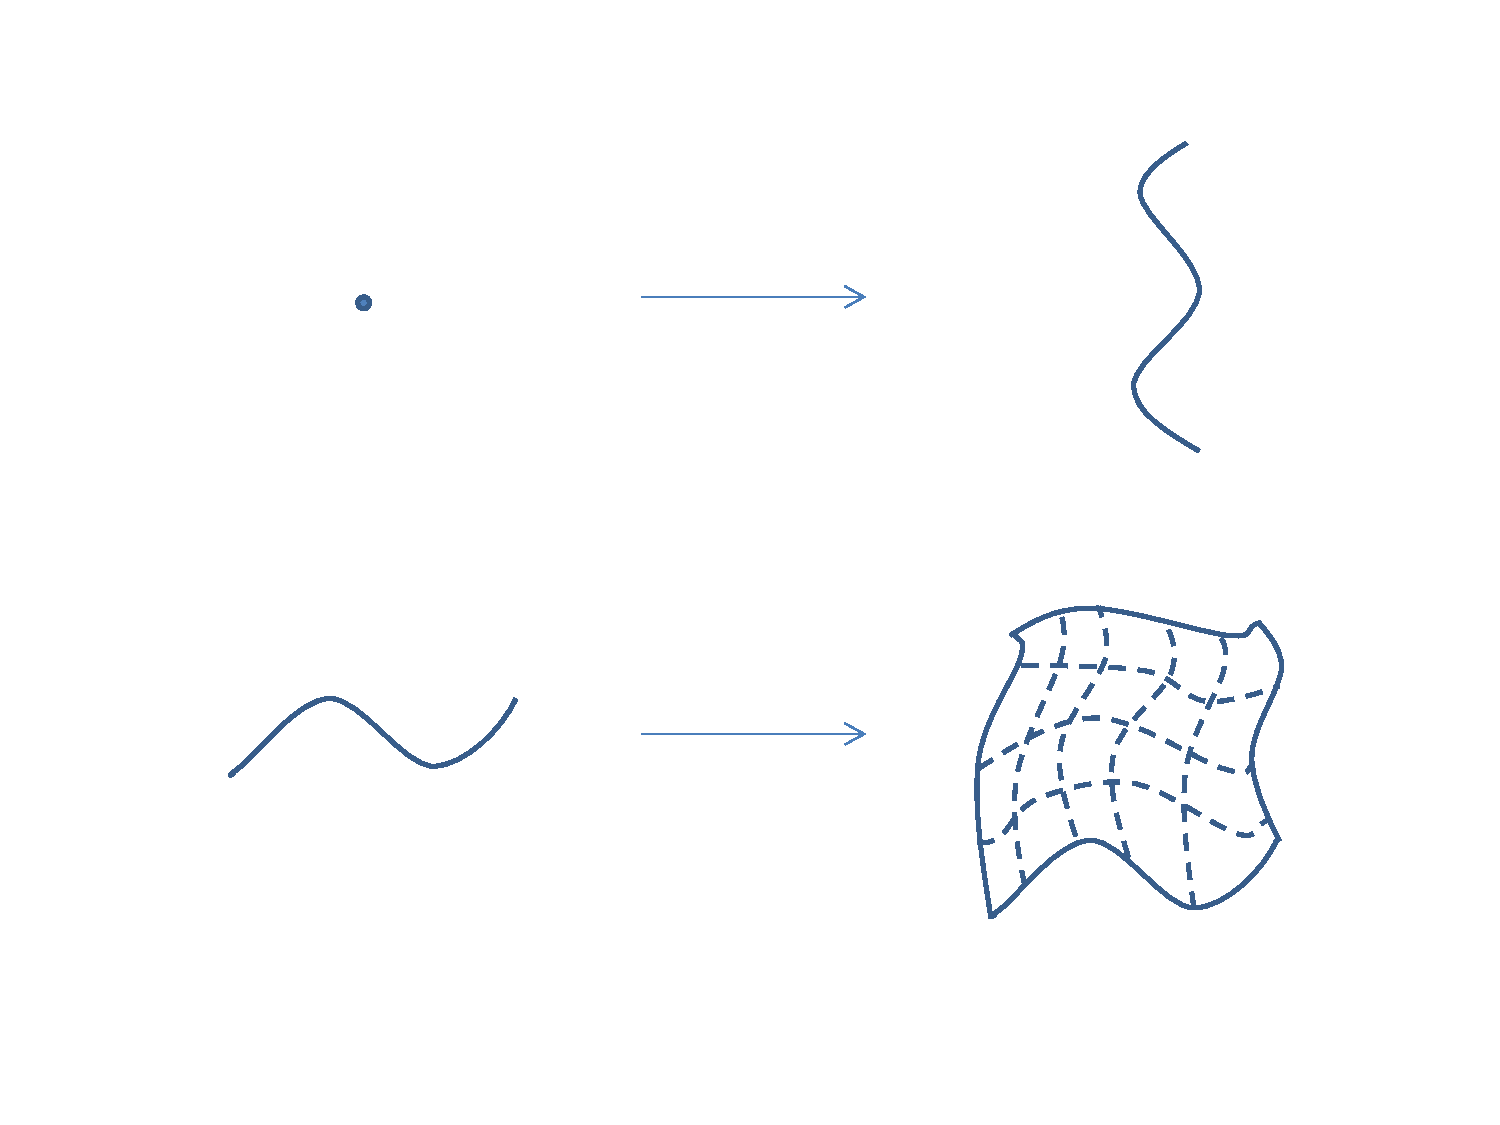
\includegraphics[width=\linewidth]{worldline2.pdf}
\end{frame}


\begin{frame}
\frametitle{String Theory as a Theory of Everything}

\begin{enumerate}
\item{Lorentz Invariance - Holds by construction}
\item{Quantisation - Holds by construction}
\item{Gravity - Appears as emergent phenomenon}
\end{enumerate}

\end{frame}

\section{Overview of the Project}

\begin{frame}
\frametitle{GGRT: The Seminal Paper}
Peter Goddard, Jeffrey Goldstone, Claudio Rebbi, Charles Thorn, \emph{Quantum Dynamics of the Massless Relativistic String}, 1972, Nuclear Physics B56 109-135
\end{frame}

\begin{frame}
\frametitle{Equations of Motion}
\begin{itemize}
\item{Classical, non-relativistic action}
\begin{itemize}
\item {fails to satisfy Lorentz invariance}
\end{itemize}
\item{Classical, relativistic action}
\begin{itemize}
\item{leads to the equations of motion}
\end{itemize}
\end{itemize}
\begin{eqnarray*}
\frac{\partial}{\partial \tau}\left( \frac{T_0}{c}\left( \frac{(\dot{X}.X')X'_\mu - (X')^2\dot{X}_\mu}{\sqrt{(\dot{X}.X')^2 - (\dot{X})^2(X')^2}}\right)\right)&&\\ + \frac{\partial}{\partial \sigma}\left(\frac{T_0}{c}\left( \frac{(\dot{X}.X')\dot{X}_\mu - (X')^2X'_\mu}{\sqrt{(\dot{X}.X')^2 - (\dot{X})^2(X')^2}}\right)\right) &=& 0
\end{eqnarray*}
\end{frame}


\begin{frame}
\frametitle{The Light-Cone Gauge}
\begin{itemize}
\item{A preferred choice of direction}
\item{+ Direction}
\begin{itemize}
\item{$(1,\, 1,\, 0\, \dots\, 0)$}
\end{itemize}
\item{- Direction}
\begin{itemize}
\item{  $(1,\, -1,\, 0\, \dots\, 0)$}
\end{itemize}
\item{Can rewrite $x^\mu$ by $(x^+,\, x^-,\, x^2,\, x^3\,\dots\,x^{d-1})$}
\end{itemize}
\end{frame}

\begin{frame}
\frametitle{Classical Equations of Motion}

\begin{eqnarray*}
X^+(\tau, \sigma) &=& 2\alpha'p^+ \tau \\
X^-(\tau, \sigma) &=& x_0^- + \sqrt{2\alpha'} \alpha_0^- \tau + i\sqrt{2\alpha'}\sum_{n=0}^\infty \frac{1}{n} \alpha_n^- e^{-in\tau} \cos n\sigma\\
X^i (\tau, \sigma) &=& x_0^i + \sqrt{2\alpha'} \alpha_0^i \tau + i\sqrt{2\alpha'}\sum_{n=0}^\infty \frac{1}{n} \alpha_n^i e^{-in\tau} \cos n\sigma\\
\text{where} \,\, \alpha^-_n&=& \frac{1}{2p^+\sqrt{2\alpha'}}\sum_{a \in \mathbb{Z}}\sum_{i=2}^{d-1}\alpha^i_{n-a}\alpha^i_a.
\end{eqnarray*}

\end{frame}

\begin{frame}
\frametitle{Quantum Equations of Motion}

\begin{eqnarray*}
\hat{X}^+(\tau, \sigma) &=& 2\alpha'\hat{p}^+ \tau \\
\hat{X}^-(\tau, \sigma) &=& \hat{x}_0^- + \sqrt{2\alpha'} \hat{\alpha}_0^- \tau + i\sqrt{2\alpha'}\sum_{n=0}^\infty \frac{1}{n} \hat{\alpha}_n^- e^{-in\tau} \cos n\sigma\\
\hat{X}^i (\tau, \sigma) &=& \hat{x}_0^i + \sqrt{2\alpha'} \hat{\alpha}_0^i \tau + i\sqrt{2\alpha'}\sum_{n=0}^\infty \frac{1}{n} \hat{\alpha}_n^i e^{-in\tau} \cos n\sigma\\
\text{where} \,\, \hat{\alpha}^-_n&=& \frac{1}{2\hat{p}^+\sqrt{2\alpha'}}\sum_{a \in \mathbb{Z}}\sum_{i=2}^{d-1}\hat{\alpha}^i_{n-a}\hat{\alpha}^i_a.
\end{eqnarray*}

\end{frame}

\section{Extra Dimensions}
\begin{frame}
\frametitle{Possible Existence of Hidden Dimensions}
\begin{itemize}
\item{Bosonic string theory predicts 26 spacetime dimensions}
\item{More modern string theories predict 10 or 11 spacetime dimensions}
\item{Trapped subspace}
\item{Compact dimensions}
\end{itemize}
\end{frame}

\begin{frame}
\frametitle{The Square Well Problem}
\begin{itemize}
\item{One dimensional space}
\item{Infinite potential outside $(0, a)$}
\item{Zero potential inside $(0, a)$}
\item{Schr\"{o}dinger equation}
\begin{itemize}
\item{ $-\frac{\hbar^2}{2m}\frac{\partial^2 \psi}{\partial x^2} = E\psi
$}
\end{itemize}
\item{Solutions}
\begin{itemize}
\item{ $\psi^p(x) = b_p \sin\frac{p\pi x} {a}$}
\end{itemize}
\item{Energies}
\begin{itemize}
\item{$E_p = \frac{\hbar^2 p^2 \pi^2}{2ma^2}$}
\end{itemize}
\end{itemize}
\end{frame}

\begin{frame}
\frametitle{Small compact dimensions}
\begin{itemize}
\item{Two-dimensional spacetime}
\begin{itemize}
\item{One observed, normal dimension, $x$}
\item{One compact hidden dimension, $y$, of length $2\pi r$}
\end{itemize}
\item{Zero potential for $x\in(0, a)$}
\item{Infinite potential for $x \notin (0, a)$}
\end{itemize}
\end{frame}

\begin{frame}
\frametitle{Small compact dimensions}
\begin{itemize}
\item{Schr\"{o}dinger equation}
\begin{itemize}
\item{$-\frac{\hbar^2}{2m}(\frac{\partial^2\psi}{\partial x^2} + \frac{\partial^2 \psi}{\partial y^2})=E\psi$}
\end{itemize}
\item{Assume $\psi(x,y) = \phi_1(x)\phi_2(y)$}
\item{By separation of variables}
\begin{itemize}
\item{$-\frac{\hbar^2}{2m}\frac{d^2\phi_1}{dx^2} = E_1\phi_1(x)$}
\item{$-\frac{\hbar^2}{2m}\frac{d^2\phi_2}{dy^2} = E_2\phi_2(y)$}
\end{itemize}
\item{Solutions}
\begin{itemize}
\item{$\phi_1^p(x) = b_p \sin \frac{p\pi x}{a}$}
\item{$\phi_2^q(y) = c_q \sin \frac{q y}{r} + d_q\cos\frac{qy}{r}$}
\end{itemize}
\end{itemize}
\end{frame}

\begin{frame}
\frametitle{Energies}
\begin{itemize}
\item{$q=0$}
\begin{itemize}
\item{$E_{p0} = \frac{\hbar^2p^2\pi^2}{2ma^2}$}
\end{itemize}
\item{q = 1}
\begin{itemize}
\item{$E_{p1} = \frac{\hbar^2}{2m}(\frac{p^2\pi^2}{a^2} + \frac{1}{r^2})$}
\end{itemize}
\item{Scales based off scale of $a$ and $r$}
\end{itemize}
\end{frame}
\section{References}
\begin{frame}
 \frametitle{References}
\begin{itemize}
\item{Peter Goddard, Jeffrey Goldstone, Claudio Rebbi, Charles Thorn, \emph{Quantum Dynamics of the Massless Relativistic String}, 1972, Nuclear Physics B56 109-135
}
\item{Barton Zwiebach, \emph{A First Course in String Theory}, 2009, Cambridge University Press }
\end{itemize}
\end{frame}


\end{document}
